%!TEX root = main.tex

%\IEEEraisesectionheading{\section{Introduction}}
\section{Introduction}
\label{sec:intro}
With a user base of more than one-tenth of the world's population,
spreadsheets are by far the most popular medium for ad-hoc exploration
and analysis of data by end-users~\cite{excel-users}. 
\saj{Studies show that information workers prefer to operate on their data within spreadsheets while shunning enterprise solutions 
with more advanced analytical features~\cite{chan1996use,raden2005shedding}. 
One popular joke among those developing business intelligence applications is that  the ``export to excel'' button is the third-most commonly used button from the menu bar, after OK and Cancel~\cite{bakke2016expressive}.}
Spreadsheets enable users to view, structure, and present data
in an intuitive tabular layout, wherein users can map their data and tasks;
this tabular layout is essential to
the popularity of spreadsheets~\cite{nardi1990spreadsheet}.

Using this tabular layout effectively involves
navigation, \ie
{\em ``the process of viewing and manipulating the computer display to
show another portion of the information space''}~\cite{nav-study}.
Navigation is supported
via two unit operations, scrolling and steering.
\saj{Scrolling is the action of moving displayed text or graphics up, down, or across a computer screen, in order to view different parts of the spreadsheet.}
For example, when analyzing data, users may scroll
to compare data across different screens, or to get
a high-level view of the overall spreadsheet.
\saj{Steering, on the other hand, involves clicking the left mouse button and then dragging the mouse pointer through the spreadsheet to select a specific region.} For example, to issue a formula,
users may steer to select
the subset of the data
to be operated on as an argument within the formula.
Most frequently used spreadsheet formulae
require users to perform steering actions~\cite{bradbard2014spreadsheet, lawson2009comparison}.
Overall, both scrolling and steering are crucial as
users navigate spreadsheets to
identify, compare, and summarize data.

\begin{figure*}
     \centering %trim=left bottom right top
  %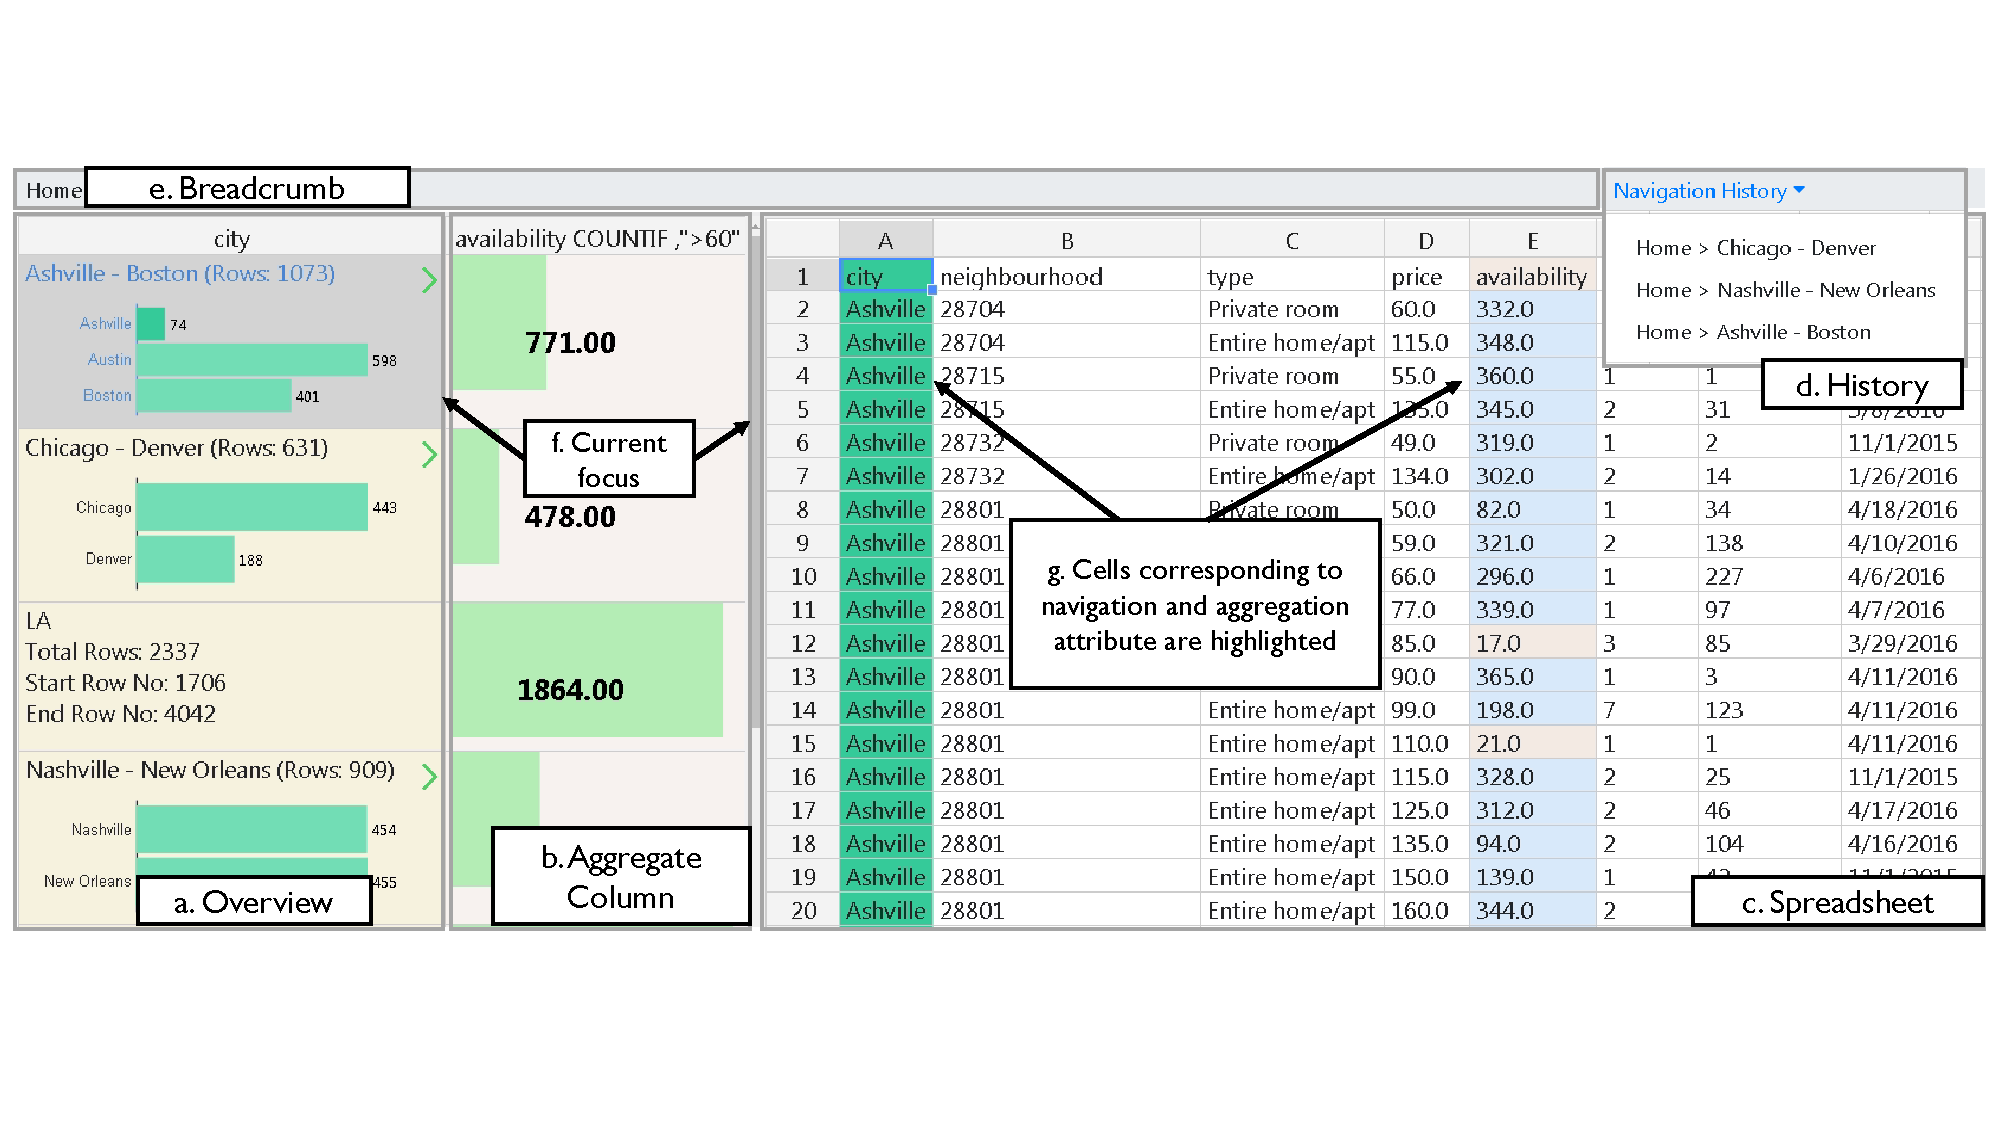
\includegraphics[width=\linewidth,trim={0 95 0 80},clip]{images/navigation.pdf}
  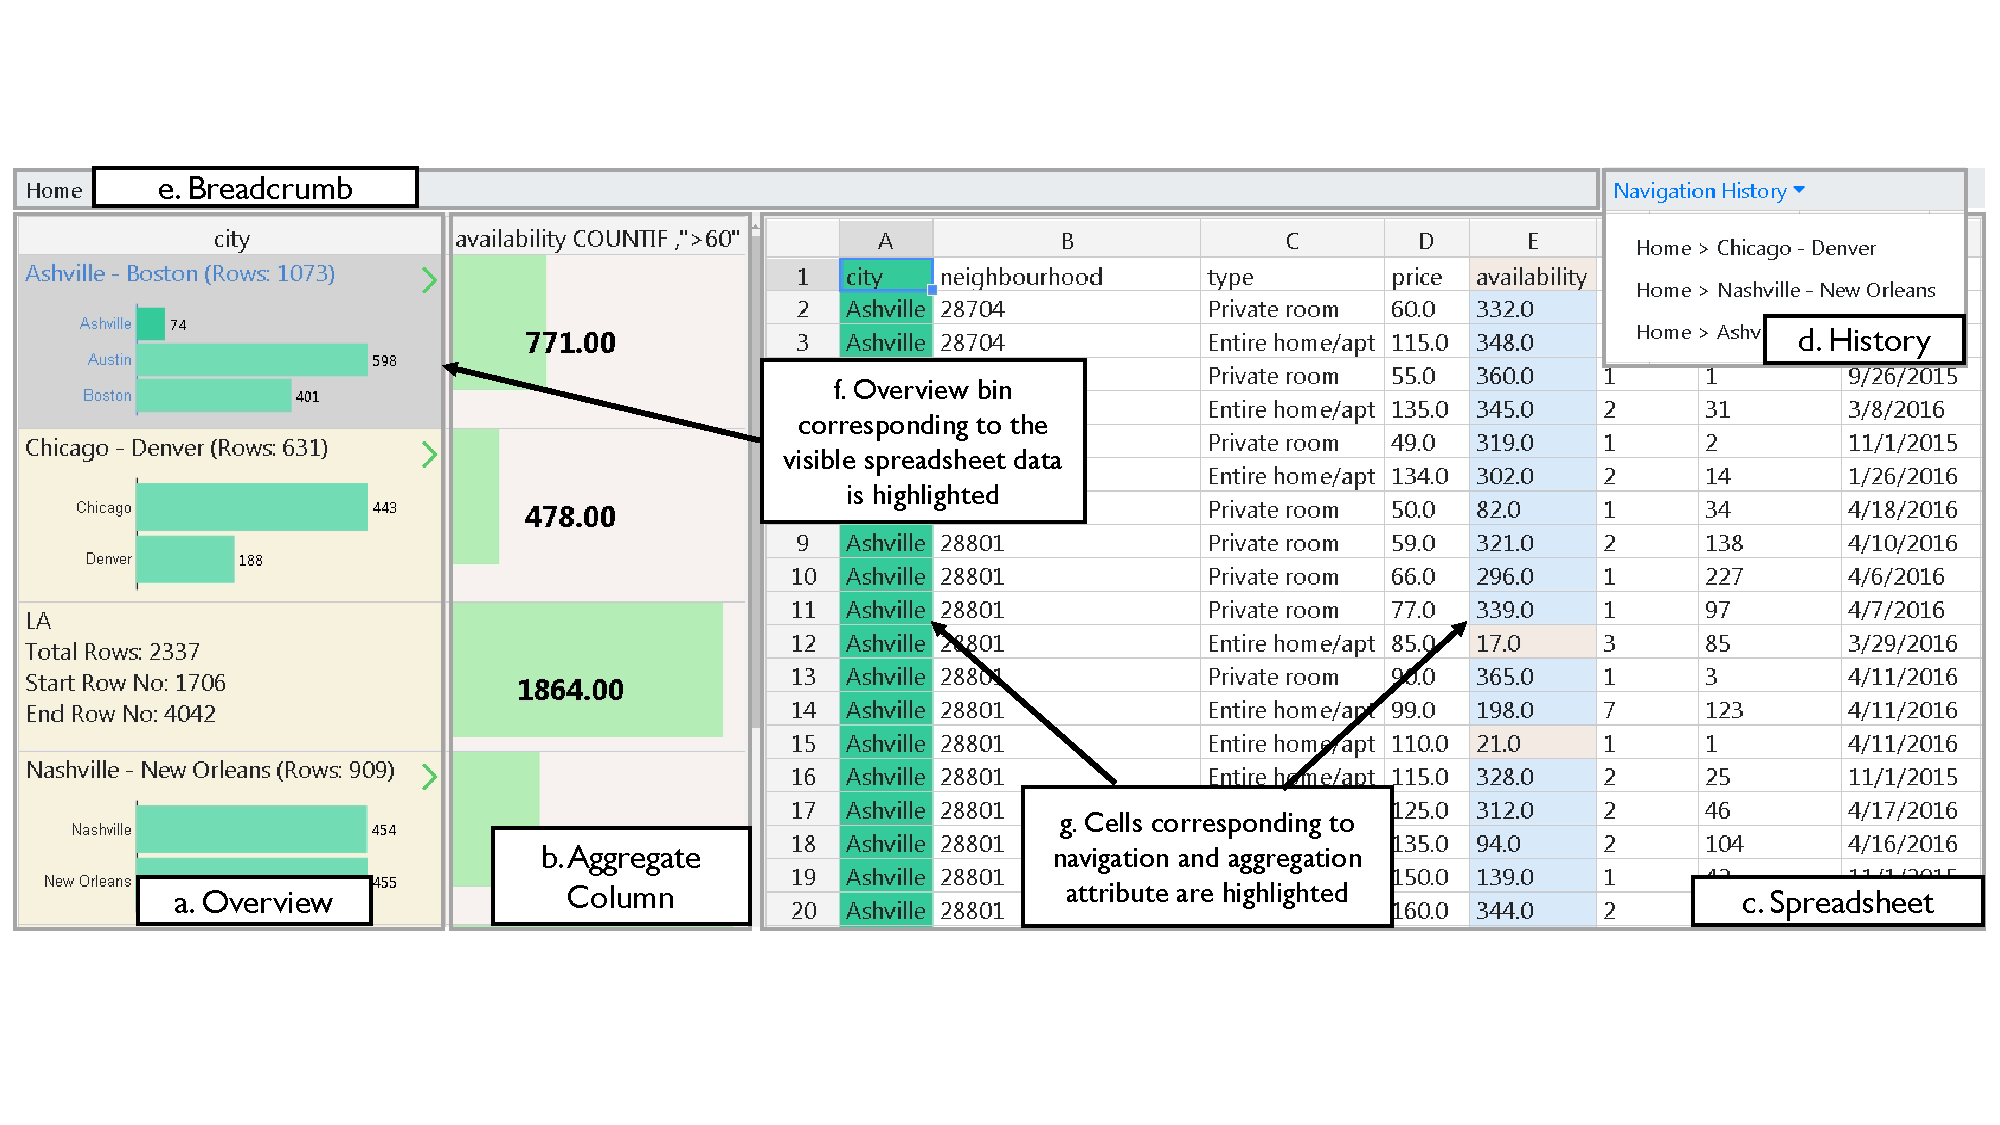
\includegraphics[width=\linewidth,trim={0 95 0 80},clip]{images/screenshot.pdf}
    \caption{\noah: navigation interface consisting of (a) a zoomable overview and (b) an aggregate column integrated with (c) a spreadsheet. A context bar consisting of (d) a navigation history displaying locations visited so far using the overview, and (e) a breadcrumb showing the current navigation path (\eg Home). (f) The user’s current focus in the spreadsheet is highlighted on the overview. (g) Columns corresponding to the navigation attribute (city) and aggregate column (availability) are highlighted on the spreadsheet.}
  \label{fig:ux}
\end{figure*}

\new{
However, navigating spreadsheets using scrolling or steering
is challenging, since spreadsheet data span multiple screens,
making it hard to synthesize, analyze, makes sense of, or
operate on it~\cite{network-context,nardi1990spreadsheet}.
With the ease of data generation, and with spreadsheets
now supporting increasingly larger datasets, \eg Google Sheets
now supports two million cells~\cite{}, a five-fold increase
from the previous limit of 400K cells, 
{\em navigating
data within spreadsheets is only becoming even harder},
thanks to
multiple inter-related reasons: 
}
\squishlist
\item {\em Loss of overview and context.}
When navigating
spreadsheets, users can easily lose the context
of where they are and where they should go next~\cite{network-context}.
The only navigational context provided by spreadsheets
is the built-in scrollbar that acts as a one-dimensional
overview and indicates the user's current location on the sheet.
However, since this overview does not capture the
layout and structure of the data,
users are forced to mentally assimilate
the layout and recall it on-demand, as they navigate a spreadsheet.

\item {\em Cognitive and mechanical burdens.}
The lack of contextual cues leads to severe
cognitive and mechanical burdens
for users~\cite{cockburn2009review}.
Users often end up taking their own drastic measures to
avoid getting lost; for example,
some users create personalized overviews
extrinsic to the spreadsheet,
by sketching maps
of spreadsheets on paper~\cite{network-context}.
Other users add their own landmarks such as headers or
colored cells, as a visual affordance to assist
in navigation~\cite{network-context}.
Steering via dragging the mouse pointer across multiple screens to select
a subset of data as input to a formula
can often be challenging as well:
the only remedy is for users to abandon steering entirely and
instead remember the range of
the subset of data of interest, and then correctly enter this range
as the argument to the formula, often giving rise to errors that are increasingly prevalent in spreadsheets~\cite{panko1998we}.


\item {\em Visual discontinuities.}
The limited viewport afforded to the user
introduces a visual discontinuity between the
information being displayed.
For example, comparing spatially separated subsets
of data within the spreadsheet
requires moving back and forth between multiple viewports,
which can be overwhelming~\cite{nardi1990spreadsheet,network-context}.
As an alternative, users tend to copy subsets of data side by side to
reduce the visual discontinuity~\cite{nardi1990spreadsheet,network-context},
which is cumbersome.
\squishend

\noindent
Overall,  while navigating present-day spreadsheets, 
{\bf \em users often lose context,
get overwhelmed, and experience visual discontinuities.} 
Addressing these challenges requires considerable manual effort.
As we \new{will} argue in Section~\ref{sec:related},
existing spreadsheet features such as
pivot tables, named ranges, and subtotals,
\new{partially alleviate 
some of the aforementioned 
challenges but do not eliminate them entirely.
For example, pivot tables generate a summary
while losing the correspondence between the
raw data and the summary, while named ranges require users
to manually associate names with ranges of data.}


So, how do we support more effective navigation of data
within spreadsheets?
One approach would be to try to integrate
an overview of the overall structure of the data along
with the spreadsheet~\cite{grudin2001partitioning}
\new{resulting in} a classical
overview+detail interface
where the spreadsheet is the detailed view.
Overview+detail interfaces are used
to facilitate navigation in various domains such as 
text editors and maps~\cite{cockburn2009review}.
\new{Users can manipulate
the overview or detailed view,
to perform high-level or low-level operations,
respectively.}
Overview+detail interfaces
have been shown to be effective in these domains,
reducing cognitive load for users by
providing \new{them} the big picture first,
helping them quickly assimilate 
the information space~\cite{cockburn2009review}.
\agp{got until here}
\saj{In this paper, our goal is to integrate an overview plug-in with spreadsheets that captures the overall structure of the data while allowing interactions that minimize the difficulties caused by typical navigational operations like scrolling and steering.}

However, while an overview plug-in for spreadsheets
does seem appealing and natural,
developing it leads to several challenges.

\squishlist
\item {\em Overview modality.}
\saj{One approach for an overview is to simply add a
zoomed out version of the entire sheet as a pane on the side,
as in popular presentation software applications like Microsoft PowerPoint or text editors
like Sublime Text. 
Unfortunately, this approach
would not suffice for a spreadsheet---while it would help users make
somewhat more informed
scrolling decisions, the zoomed out presentation of the overview would be unreadable. An overview should provide a comprehensible big picture view of the spreadsheet.
Another approach, adopted by map tools like the
early versions of Google maps,
is to use the overview
to provide a global context of the user's current location
being displayed in the zoomed in detailed view~\cite{cockburn2009review}.
While the overview remains static, users can perform semantic zooming operations~\cite{perlin1993pad} on the detailed
view which allows objects to be represented differently at different scales. Since spreadsheets already display the raw data,
zooming into and out of a detailed view consisting of
this raw data is not meaningful. Rather, the spreadsheet overview should dynamically change as users sought more fine-grained or coarse-grained view of the overall structure of the data.} 

\item {\em Construction of the overview.}
\saj{Given a spreadsheet
with many rows, 
one approach to constructing a dynamic overview is mapping rows of data to high level groups similar to online maps. In online maps, cities are grouped into states and states are grouped into countries forming a multi-granularity hierarchy. How do we automatically group spreadsheet rows together in a similar ``meaningful''
way
such that this grouping applies to all 
data types, including strings and numbers? If the automatic grouping is not meaningful, how do we allow the users
to customize the overview
to construct meaningful groups? How do we facilitate interactions that enable users view the overview at multiple granularities?}

\item {\em Operations on the overview.}
\saj{Following the construction of a dynamic overview, the next challenge is to design simple interactions that achieve similar outcomes as scrolling and steering.
For example, an alternative to scrolling can be to leverage the groups of the overview to access the rows mapped to that group. How do we leverage the overview so that users can perform similar simple interaction to steer spreadsheet data and issue formula? As the granularity of the dynamic overview changes, how do we efficiently update the mapping from spreadsheet rows to the finer or coarser groups so that scrolling remains seamless? How do we recompute the results of a formula as the granularity changes without requiring the users to reissue the formula from scratch? How do we ensure such automatic recomputation scales with the size of the data?}

\item {\em Seamless integration as a plug-in.}
Finally, the design of the overview
should be generic so that it can be integrated
with any existing spreadsheet tool on any spreadsheet
dataset without impacting
existing functionalities or look-and-feel.
Any new interactions introduced should be consistent
with traditional spreadsheet semantics,
and complement existing spreadsheet interactions.
Interactions between the overview and the raw spreadsheet
should be coordinated to the extent possible.
\squishend

\begin{comment}
Since we want to allow users to control how the overview
is constructed, we can let them select the grouping
attribute(s). Following this, we need mechanisms to automatically group nearby rows
into meaningful bins.
This necessitates
{\em semantic zooming}~\cite{perlin1993pad} instead of geometric
zooming (unlike text editors or presentation software),
on the overview view instead of the detailed view
(unlike map tools).
Several domains, \eg online maps and program visualization,
adopt semantic zooming
to ensure improved readability and
comprehension of the information displayed~\cite{summers2003experimental}.
However, to the best of our knowledge, no prior work
has ever developed semantic zooming for spreadsheet data.
Customizing these bins will also eliminate
visual discontinuities: users can simply arrange the bins
the way they want and keep them near each other
for easy comparison.
For this, we take inspiration from aggregation
in relational databases. In relational databases, each ``group'' is associated
with one or more aggregates. As long as the groups are
appropriately constructed (using the mechanisms alluded to above),
formulae can be issued once without requiring any steering, and
automatically maintained for all groups when
zooming in and zooming out. 
\end{comment}

\stitle{\noah.} We address the aforementioned challenges
in our tool \noah,
an in-situ
\textbf{\underline{n}}avigation interface
for \textbf{\underline{o}}verviewing
and \textbf{\underline{a}}nalyzing
spreadsheet data \textbf{\underline{h}}olistically.
\noah is constructed as a plugin to
an existing spreadsheet tool,
{\scshape DataSpread}~\cite{dataspread},
an open-source scalable web-based spreadsheet.
While \noah's design is not tied to {\sc DataSpread},
we opted not to use other popular spreadsheet
tools like Google Sheets and Microsoft Excel because they
are closed source.
Figure~\ref{fig:ux} shows a snapshot of \noah.
When the user chooses to explore
the data by a specific attribute,
\saj{a multi-granularity overview is constructed and displayed
within \noah, next to the raw spreadsheet data (Figure~\ref{fig:ux}a). Users can zoom into or out of the overview to obtain a fine-grained or coarse grained perspective of the data distribution. The distribution at each granularity is captured by a histogram,
enabling users to assimilate the data. Each bin (group) of the histogram is mapped to a collection of rows in the spreadsheet.} Cumbersome scrolling operations are eliminated in favor
of a few clicks on the overview interface. Instead of steering to analyze the data,
users can issue formulae
on the overview with interactions similar to pivot table construction,
and view results on a separate {\em aggregate column},
alongside the overview (Figure~\ref{fig:ux}b). 
In this manner,
users can issue formulae on different
subsets of the data while remaining on the same screen,
reducing visual discontinuity.
\noah ensures that there is coordination between
the overview and the spreadsheet:
for example, panning and zooming on the overview
are reflected on the spreadsheet by displaying
the spreadsheet data corresponding to the bin
currently in focus in the overview.
Finally, \noah automatically creates
contextual and historical information
(Figure~\ref{fig:ux}d and~\ref{fig:ux}e)
while displaying visual cues
(Figure~\ref{fig:ux}f and~\ref{fig:ux}g)
so that users don't lose context during navigation.

The primary contribution of our work is twofold:
\squishlist
\item We formalize the design of a general
navigation (overview+detail) interface
for exploration and analysis of large spreadsheets.
We realize this design in the form of \noah,
a plugin to an existing web-based spreadsheet tool,
ensuring that interactions supported by \noah
complement existing spreadsheet operations.
\item We conduct a user study to evaluate
the benefits and limitations of this plugin.
\saj{The study shows that compared to Microsoft Excel, participants were able to complete spreadsheet
tasks involving navigation 
correctly and quickly in \noah. Participants made {\bf $2.5\times$ fewer} mistakes while being {\bf $2\times$ faster} with a \noah-integrated spreadsheet than with Excel.} 
\squishend


\toappendix{The rest of the paper is organized as follows: In Section~\ref{sec:usage} we first present a case study of \noah being applied to a real-world scenario.  
In Section~\ref{sec:related}, we discuss related work. We then explain the design considerations for developing \noah in Section~\ref{sec:design}. In Section~\ref{sec:ui}, we present \noah’s user interface and supported operations. We then discuss the design and outcomes of a user study evaluating the effectiveness of \noah in Section~\ref{sec:study}. Finally, we discuss the limitations of \noah and possible future enhancements in Section~\ref{sec:discuss}.}

\section{\noah Use Cases}
\label{sec:usage}
\saj{As explained in Section~\ref{sec:intro}, users prefer spreadsheets over enterprise solutions to view, directly manipulate, and explore data~\cite{chan1996use,raden2005shedding}. To identify the scope of these tasks on spreadsheets (see Table~\ref{tab:scope}), we draw parallel to the typology of abstract data exploration tasks~\cite{brehmer2013multi}. The typology characterizes the exploration and manipulation tasks performed on visual representations of data. While all the tasks in Table~\ref{tab:scope} can be performed using spreadsheets, \noah enhances the experience for a subset of these tasks, indicated by a checkmark (\checkmark). We explain how \noah complements spreadsheets in accomplishing these tasks in Appendix.}

\begin{table}[!htb]\scriptsize
\caption{Uses cases of \noah.}
\label{tab:scope}
\centering
\begin{tabular}{c c}
\hline
Purpose & Use Cases   \\ \hline
\emph{Consume}         & \code{discover} (\checkmark), \code{present} (\checkmark), \code{enjoy} (\checkmark)\\
\emph{Produce}         & \code{create} (\checkmark), \code{annotate} ($\times$)\\
\emph{Search}            & \code{browse} (\checkmark), \code{explore (\checkmark)}, \code{locate} ($\times$), \code{lookup} ($\times$)\\
\emph{Query}    &  \code{identify} (\checkmark), \code{summarize} (\checkmark), \code{compare} (\checkmark)  \\ \hline
\end{tabular}
\end{table}

\saj{We now describe a usage scenario that captures the spreadsheet exploration tasks accommodated by \noah (Table~\ref{tab:scope}) while illustrating the benefits of integrating an overview with spreadsheets. Let's assume that} Rebecca, an investigative journalist
is exploring the Inside Airbnb dataset~\cite{web:airbnb},
a dataset of all the Airbnb listings across different US cities.
This dataset was created to investigate the long-standing
accusation that many listings in Airbnb are illegally
run as hotel businesses, while avoiding taxes;
any listing available for rent for more than $60$ days
a year is considered to be operated as a hotel~\cite{accusation}. 

Without any prior knowledge of the dataset,
Rebecca starts by finding out information
about cities in the dataset and their corresponding listings;
for example, which cities are present,
and roughly how many listings does each city have \saj{(\code{browse} and \code{explore})}.
Without \noah, Rebecca may have used
a pivot table (discussed in Section~\ref{sec:related})
to construct
a summary---however, since this summary is disconnected
from the underlying data, it is hard for Rebecca to
map the summary statistics to
the raw data to obtain further details
about listings from any given city.
If she wanted to identify listings from a specific city \saj{(\code{lookup} and \code{locate} or \code{identify})},
Rebecca would have to either use search capabilities or
perform an explicit filter for this information,
and would have to switch back and forth between the
pivot table results and the raw listings,
present at disparate locations
on the spreadsheet.
Even at the first step of this exploration,
Rebecca would experience substantial cognitive burden,
loss of context,
and visual discontinuities,
with subsequent steps becoming progressively
more challenging.


Using \noah, she explores
the data by city,
with \noah providing a high-level overview of
cities (Figure~\ref{fig:ux}a).
The overview consists of sorted non-overlapping bins
containing one or more cities.
She can click on any bin and the corresponding
data will be displayed at the top of her screen.
For example, clicking on the {\em Ashville-Boston} bin
displays the Ashville listings (Figure~\ref{fig:ux}c).
She can also zoom into bins using the ``\textcolor{blue}{$\rangle$}'' arrows,
zoom out of bins using the ``\textcolor{blue}{$\langle$}'' arrows,
and pan by clicking on various bins at the same level.
We discuss the construction of the overview
and associated interactions in Section~\ref{sec:ui}.


Next, say Rebecca wants to analyze
one of the larger cities \saj{(\code{query}/\code{summarize}) to understand the renting pattern}.
She identifies these cities by
comparing the number of listings
for each city displayed on the overview \saj{(\code{compare})}.
She decides to focus on Boston, her hometown,
and wants to find out how many listings
in Boston violate
the ``rent availability $>60$ days'' condition.
In a typical spreadsheet, Rebecca needs to manually steer and then select
the Boston listings as input to a \code{COUNTIF} formula that counts the number of
rows that satisfy the above mentioned condition.
Using \noah, she can zoom into
the {\em Ashville-Boston} bin
(Figure~\ref{fig:concept}a and~\ref{fig:concept}b)
and then issues
a \code{COUNTIF} operation on the overview.
%\ie a \code{COUNTIF} formula\footnote{\code{COUNTIF} is a
%type of formula in spreadsheets that counts the number %of
%rows that satisfy some condition.}. 
The result is displayed as an {\em aggregate column}
alongside the overview (Figure~\ref{fig:ux}b).
Rebecca learns \saj{(\code{discover})} that more than half of the listings in Boston are 
effectively operating as hotels---a large number! 

Based on this insight, Rebecca then wants to
understand availability statistics for an even
larger city, Chicago \saj{(\code{summarize})}.
As she uses the overview to navigate
to Chicago, \noah
automatically updates the aggregate column to
the \code{COUNTIF} formula results for Chicago,
without Rebecca needing to reissue it by performing a cumbersome steering operation as in traditional spreadsheets. 
Rebecca learns that Chicago exhibits 
a similar renting pattern as Boston, with more than half the listings operating as hotels. She can then check if this trend holds for all large cities \saj{(\code{compare})},
and whether the smaller cities have a different pattern \saj{(\code{discover})}. \saj{Note that, the rows that satisfy the ``rent availability $>60$ days'' condition, are listed
 in the spreadsheet adjacent
to the overview in sky blue (Figure~\ref{fig:ux}g)}. With the raw 
data presented side-by-side, she can also dive into other attributes
of the listings operating as hotels to see if there are any other identifying characteristics,
\eg if they are all managed by a small number of agencies acting as individual renters \saj{(\code{identify})}.

 Finally, as Rebecca navigates the data,
 her navigation history (Figure~\ref{fig:ux}d),
 \ie recently visited cities, and current navigation path
 (Figure~\ref{fig:ux}e) are kept up-to-date,
 allowing her to maintain context during navigation.
 She can revisit any previously visited cities
 by simply clicking on the relevant path
 in the navigation history.


Overall, with \noah, users can quickly
comprehend the data via the overview, access any region 
within the data without having to
scroll endlessly, and request additional details on demand without having to
steer across multiple screens. As users navigate and analyze the data, 
they can revisit previously accessed data via the navigation history, not losing context
of what they have explored. 





